\documentclass[12pt]{book}

% ── Packages ─────────────────────────────────────────────────────────────
\usepackage[margin=1.2in]{geometry}
\usepackage{amsmath,amssymb}
\usepackage{setspace}
\usepackage{parskip}
\usepackage{titlesec}
\usepackage{hyperref}
\usepackage{tikz}
\usepackage{tikz-3dplot}
\usetikzlibrary{calc,arrows.meta,positioning,decorations.pathmorphing,patterns}
\usepackage{imakeidx}
\makeindex[name=keywords,title={Keywords Index},columns=2,columnsep=18pt]
\makeindex[name=words,title={Word Index},columns=2,columnsep=18pt]

% ── Typography ───────────────────────────────────────────────────────────
\setstretch{1.3}
\setlength{\parindent}{0pt}
\setlength{\parskip}{8pt}

\titleformat{\chapter}[display]
{\normalfont\Large\bfseries}{\chaptername\ \thechapter}{12pt}{\Huge}
\titleformat{\section}{\normalfont\large\bfseries}{\thesection}{1em}{}

% ── Teacher Notes Environment ───────────────────────────────────────────
\newenvironment{teachernote}
{\par\medskip\noindent\textbf{Teacher Note:} \itshape}
{\par\medskip}

% ── Title ────────────────────────────────────────────────────────────────
\title{\textbf{How Ideas Work}\\[6pt]
\large A Book About Rules, Patterns, and Discovery}
\author{Flyxion}
\date{}

% ════════════════════════════════════════════════════════════════════════
\begin{document}
% ════════════════════════════════════════════════════════════════════════

\maketitle
\tableofcontents

% ════════════════════════════════════════════════════════════════════════
\chapter*{Teacher's Guide}
\addcontentsline{toc}{chapter}{Teacher's Guide}
% ════════════════════════════════════════════════════════════════════════

\section*{Purpose of This Book}

This book is not only about learning\index[words]{learning} ideas\index[words]{idea}. It is about learning\index[words]{learning} how ideas\index[words]{idea}
form, how they simplify, how they become fast, and how they are tested
and repaired.

Each chapter introduces a way of thinking that can be revisited many times.
The goal is not to complete the book once, but to return to it at increasing
levels of depth as the student grows.

\section*{A Multi-Year Structure}

The material in this book can be spread across multiple grades. Each pass
through the book should deepen understanding\index[words]{understanding} rather than simply repeat it.

In early grades, students should focus on recognizing patterns\index[words]{pattern}\index[keywords]{pattern} and
participating in the demonstrations\index[keywords]{demonstration (hands-on)}. The emphasis should be on experience.

In later grades, students should begin to explain why the demonstrations\index[keywords]{demonstration (hands-on)}
work, using their own words and examples.

In advanced stages, students should begin applying these ideas\index[words]{idea} across
different subjects and identifying structure\index[words]{structure} independently.

\section*{Suggested Progression}

\subsection*{Early Stage (Younger Students)}

At this stage, the focus is on concrete experience.

Students should complete the hands-on demonstrations\index[keywords]{demonstration (hands-on)}, describe what they
notice in simple language, and recognize patterns\index[words]{pattern}\index[keywords]{pattern} when they appear. The
goal is familiarity, not precision.

\subsection*{Middle Stage (Developing Students)}

At this stage, the focus shifts to explanation.

Students should explain the demonstrations\index[keywords]{demonstration (hands-on)} in their own words, give
examples from everyday life, and begin noticing when rules\index[words]{rule}\index[keywords]{rule} agree or
conflict. The goal is understanding\index[words]{understanding} relationships between ideas\index[words]{idea}.

\subsection*{Later Stage (Advanced Students)}

At this stage, the focus is transfer\index[keywords]{transfer (of knowledge)} and creation.

Students should apply ideas\index[words]{idea} across different subjects, design their own
demonstrations, and identify patterns\index[words]{pattern}\index[keywords]{pattern} without being prompted. The goal
is independent structural thinking.

\section*{How to Use the Demonstrations}

Each chapter ends with a hands-on demonstration. These are not optional.
They are the core of the learning\index[words]{learning} process.

Teachers should allow students to attempt the activity before explaining
it, encourage students to describe what happened, and avoid giving the
answer\index[words]{answer} too early. The demonstration works best when the student discovers
the result.

\section*{Common Mistakes}

Students may try to guess answers\index[words]{answer} instead of following rules\index[words]{rule}\index[keywords]{rule}, focus on
surface details\index[words]{detail} instead of structure\index[words]{structure}, or become frustrated when rules\index[words]{rule}\index[keywords]{rule}
conflict. These are not failures\index[words]{failure}. They are part of the process.

The role of the teacher is not to remove difficulty, but to guide
attention toward what matters.

\section*{Connection to Other Subjects}

This book is designed to connect with all areas of learning\index[words]{learning}. Teachers are
encouraged to refer back to these ideas during mathematics\index[words]{mathematics} (patterns\index[keywords]{pattern},
rules\index[words]{rule}\index[keywords]{rule}, abstraction\index[keywords]{abstraction}), science (testing ideas, fixing contradictions\index[words]{contradiction}\index[keywords]{contradiction}),
language (structure\index[words]{structure}, meaning, communication), and art (form, pattern\index[words]{pattern},
transformation). The same structures\index[words]{structure} appear everywhere.

\section*{Final Note}

This book teaches a way of thinking that builds over time. Students who
revisit these ideas will begin to notice something important: solutions\index[words]{solution} do
not appear from nowhere. They emerge when enough rules\index[words]{rule} are understood at
once. That moment of recognition\index[words]{recognition}\index[keywords]{recognition} is not luck. It is the result of accumulated
structure\index[words]{structure}.

% ════════════════════════════════════════════════════════════════════════
\part{How Ideas Form}
% ════════════════════════════════════════════════════════════════════════

\chapter{The Puzzle That Solves Itself}

Have you ever been working on a puzzle\index[words]{puzzle} and suddenly, without trying, the
last piece just \emph{clicked} into place? You didn't force it. You didn't
guess. The shape of every other piece told you exactly where it had to go.

That click is what a great idea feels like.

We often think that having a brilliant idea means making something up out
of nothing---like pulling a rabbit from a hat. But most of the time, ideas
work more like puzzles\index[words]{puzzle}. The more pieces you have in place, the fewer places
the last piece can go. Eventually, there is only one place it fits.

\textbf{Big Idea:} You don't invent the solution\index[words]{solution}. The solution\index[words]{solution} becomes the
only thing that works.

\begin{quote}\itshape
If you try every wrong piece first, the last one will always feel like a
miracle. It isn't. It's just the only piece left.
\end{quote}

% ── Chapter 1 Figure ─────────────────────────────────────────────────────
\begin{figure}[h!]
\centering
\tdplotsetmaincoords{68}{118}
\begin{tikzpicture}[tdplot_main_coords, scale=2.2, line join=round, line cap=round]
% outer cube
\coordinate (O) at (0,0,0);
\coordinate (A) at (2,0,0);
\coordinate (B) at (2,2,0);
\coordinate (C) at (0,2,0);
\coordinate (D) at (0,0,2);
\coordinate (E) at (2,0,2);
\coordinate (F) at (2,2,2);
\coordinate (G) at (0,2,2);
\draw[thick] (O)--(A)--(B)--(C)--cycle;
\draw[thick] (D)--(E)--(F)--(G)--cycle;
\draw[thick] (O)--(D) (A)--(E) (B)--(F) (C)--(G);
% slices
\fill[blue!12] (1.2,0,0)--(2,0,0)--(2,2,0)--(1.2,2,0)--cycle;
\fill[blue!12] (1.2,0,2)--(2,0,2)--(2,2,2)--(1.2,2,2)--cycle;
\draw[dashed,blue!70] (1.2,0,0)--(1.2,0,2) (1.2,2,0)--(1.2,2,2)
  (1.2,0,0)--(1.2,2,0) (1.2,0,2)--(1.2,2,2);
\fill[red!12] (1.2,1.1,0)--(2,1.1,0)--(2,2,0)--(1.2,2,0)--cycle;
\fill[red!12] (1.2,1.1,2)--(2,1.1,2)--(2,2,2)--(1.2,2,2)--cycle;
\draw[dashed,red!70] (1.2,1.1,0)--(1.2,1.1,2) (2,1.1,0)--(2,1.1,2)
  (1.2,1.1,0)--(2,1.1,0) (1.2,1.1,2)--(2,1.1,2);
\fill[green!12] (1.7,1.1,0)--(2,1.1,0)--(2,2,0)--(1.7,2,0)--cycle;
\fill[green!12] (1.7,1.1,2)--(2,1.1,2)--(2,2,2)--(1.7,2,2)--cycle;
\draw[dashed,green!60!black] (1.7,1.1,0)--(1.7,1.1,2) (1.7,2,0)--(1.7,2,2);
% final point
\filldraw[black] (1.85,1.75,1.2) circle (1.2pt);
\node[anchor=west] at (2.15,1.8,1.2) {\small only one fit left};
\node at (1,-0.45,0) {\small many possibilities};
\node[blue!70] at (2.4,0.5,1.4) {\small rule 1};
\node[red!70] at (2.35,1.25,1.65) {\small rule 2};
\node[green!50!black] at (2.3,1.85,0.95) {\small rule 3};
\end{tikzpicture}
\caption{Rules shrink the space of possible answers until only one remains.}
\end{figure}

\section{Rules of the Game}

Every game\index[words]{game} has rules. In chess\index[words]{chess}, a knight moves in an L-shape. In soccer,
you cannot use your hands. In mathematics\index[words]{mathematics}, two plus two always equals four.

Rules tell you what is allowed and what is not. The more rules there are,
the fewer moves you can make.

Ideas work the same way. Every field of knowledge\index[words]{knowledge}---science, music\index[words]{music}, building,
cooking\index[keywords]{cooking}---has its own set of rules. When you learn something, you are really
learning\index[words]{learning} its rules.

\section{When Rules Stack Up}

Here is something interesting. One rule by itself does not tell you very
much. But when you put many rules together, something surprising happens:
the number of possible answers\index[words]{answer} gets smaller and smaller.

Imagine you are thinking of a number.
\begin{itemize}
\item It is between 1 and 100. (That leaves 100 possible answers\index[words]{answer}.)
\item It is even. (Now there are 50.)
\item It is greater than 90. (Now there are 5.)
\item It ends in 4. (Now there is exactly 1: 94.)
\end{itemize}

No one told you the answer\index[words]{answer}. The rules told you. When enough rules stacked
up, there was only one number left.

Ideas work exactly like this. When you have studied something long enough,
and learned enough rules from enough different places, the answer stops
being a guess. It becomes the only thing that could be true.

\section{Why It Feels Like a Surprise}

If the answer is inevitable, why does it still feel like a surprise?

Because you cannot always see all the rules at once. They are stored in
different parts of your memory\index[words]{memory}. The moment of a great idea is the moment
they all line up at the same time, and you finally see the shape they were
pointing toward all along.

This is why very experienced people often say, ``I just knew.'' They did
not guess. They had so many rules stacked up inside them that the answer
arrived the same way the last puzzle\index[words]{puzzle} piece clicks in---not with effort,
but with recognition\index[words]{recognition}\index[keywords]{recognition}.

\begin{quote}\itshape
A puzzle\index[words]{puzzle} doesn't hide the answer.
It slowly removes everything that isn't the answer.
\end{quote}

\begin{quote}\itshape
Some ideas feel small until they suddenly open up.
\end{quote}

\begin{teachernote}
This chapter introduces the central cognitive shift of the entire book:
moving from the idea of invention to the idea of constraint\index[keywords]{constraint} convergence.
Students will initially interpret the puzzle\index[words]{puzzle} example as a story about
success or cleverness. The goal is to redirect their attention toward
necessity: the answer appears because all other possibilities have been
eliminated. The number-filtering example is especially important. It should
not be treated as arithmetic practice\index[words]{practice}\index[keywords]{practice}, but as an experience of shrinking
possibility space\index[keywords]{possibility space}. Encourage students to notice how each rule reduces the
number of valid answers. If students describe the final answer as
``chosen'' or ``guessed,'' gently challenge this. Ask whether any other
answer could have worked once all rules were applied. This chapter lays
the foundation for everything that follows. If this shift is not
established, later ideas may be interpreted incorrectly as memorization
rather than structure.
\end{teachernote}

% ────────────────────────────────────────────────────────────────────────
\chapter{Learning Rules from the World}
% ────────────────────────────────────────────────────────────────────────

\section{Rules Are Everywhere}

You might think that rules only exist in school subjects like math or
science. But rules are everywhere, even in everyday life.

Whenever something works the same way again and again, there is a rule
behind it. You may not know the rule yet, but your brain\index[words]{brain} is already
collecting it.

\textbf{Big Idea:} Learning is noticing what stays the same.

\begin{quote}\itshape
If you collect enough rules, they start talking to each other
even when you are not listening.
\end{quote}

% ── Chapter 2 Figure ─────────────────────────────────────────────────────
\begin{figure}[h!]
\centering
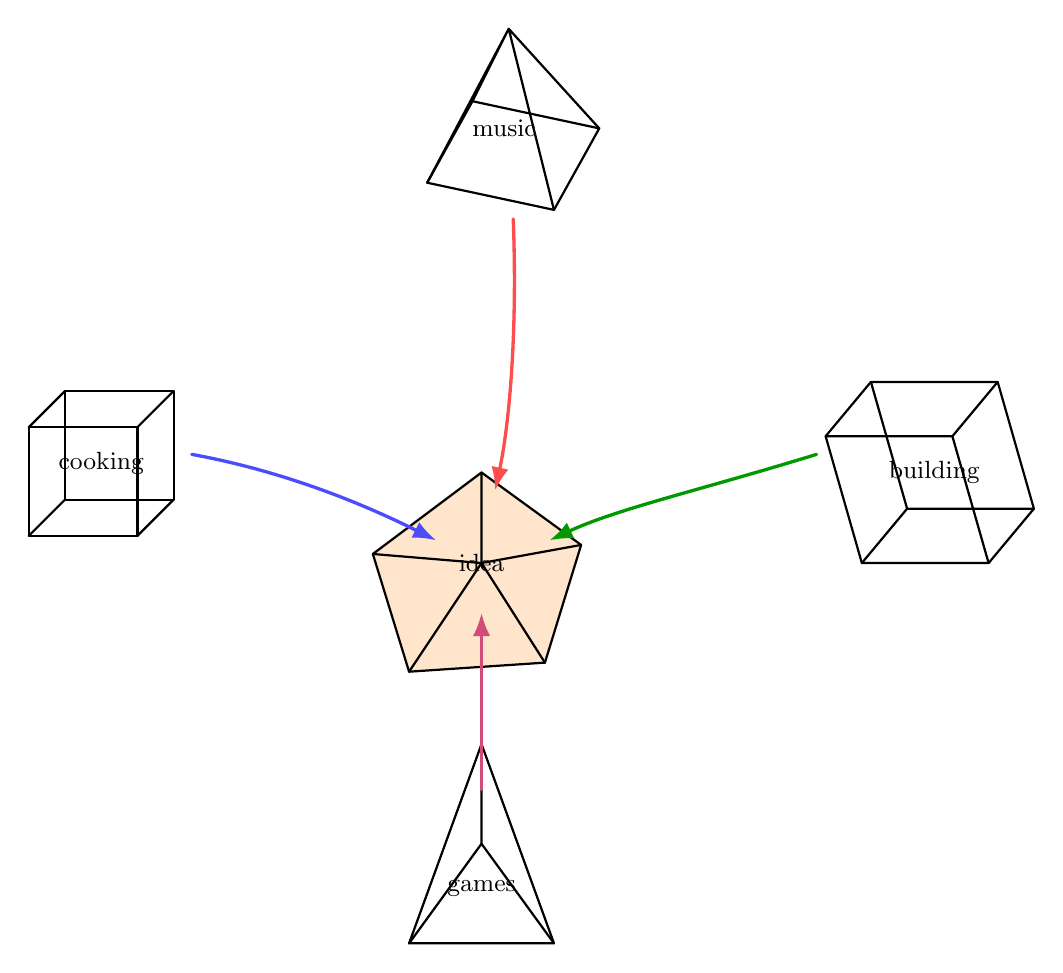
\begin{tikzpicture}[scale=1.15, line join=round, line cap=round, >=Latex]
% central polyhedron-ish core
\coordinate (M) at (0,0);
\fill[orange!20] (0,1.2) -- (1.1,0.4) -- (0.7,-0.9) -- (-0.8,-1.0) -- (-1.2,0.3) -- cycle;
\draw[thick] (0,1.2) -- (1.1,0.4) -- (0.7,-0.9) -- (-0.8,-1.0) -- (-1.2,0.3) -- cycle;
\draw[thick] (0,1.2)--(0,0.2) (1.1,0.4)--(0,0.2) (-1.2,0.3)--(0,0.2)
  (0.7,-0.9)--(0,0.2) (-0.8,-1.0)--(0,0.2);
\node at (0,0.2) {\small idea};
% left cube
\draw[thick] (-5,0.5)--(-3.8,0.5)--(-3.8,1.7)--(-5,1.7)--cycle;
\draw[thick] (-4.6,0.9)--(-3.4,0.9)--(-3.4,2.1)--(-4.6,2.1)--cycle;
\draw[thick] (-5,0.5)--(-4.6,0.9) (-3.8,0.5)--(-3.4,0.9)
  (-3.8,1.7)--(-3.4,2.1) (-5,1.7)--(-4.6,2.1);
\node at (-4.2,1.3) {\small cooking};
% top pyramid
\draw[thick] (-0.6,4.4)--(0.8,4.1)--(1.3,5.0)--(-0.1,5.3)--cycle;
\draw[thick] (0.3,6.1)--(-0.6,4.4) (0.3,6.1)--(0.8,4.1)
  (0.3,6.1)--(1.3,5.0) (0.3,6.1)--(-0.1,5.3);
\node at (0.25,5.0) {\small music};
% right prism
\draw[thick] (4.2,0.2)--(5.6,0.2)--(5.2,1.6)--(3.8,1.6)--cycle;
\draw[thick] (4.7,0.8)--(6.1,0.8)--(5.7,2.2)--(4.3,2.2)--cycle;
\draw[thick] (4.2,0.2)--(4.7,0.8) (5.6,0.2)--(6.1,0.8)
  (5.2,1.6)--(5.7,2.2) (3.8,1.6)--(4.3,2.2);
\node at (5.0,1.2) {\small building};
% bottom tetra
\draw[thick] (-0.8,-4.0)--(0.8,-4.0)--(0,-2.9)--cycle;
\draw[thick] (0,-1.8)--(-0.8,-4.0) (0,-1.8)--(0.8,-4.0) (0,-1.8)--(0,-2.9);
\node at (0,-3.4) {\small games};
% arrows
\draw[->,very thick,blue!70] (-3.2,1.4) .. controls (-2.1,1.2) and (-1.2,0.8) .. (-0.5,0.45);
\draw[->,very thick,red!70] (0.35,4.0) .. controls (0.4,2.7) and (0.3,1.7) .. (0.15,1.0);
\draw[->,very thick,green!60!black] (3.7,1.4) .. controls (2.4,1.0) and (1.5,0.8) .. (0.75,0.45);
\draw[->,very thick,purple!70] (0,-2.3) .. controls (0,-1.6) and (0,-0.7) .. (0,-0.35);
\end{tikzpicture}
\caption{Rules come from many places, but they can meet in one shared structure.}
\end{figure}

\section{Cooking: Following the Recipe Without Seeing It}

Imagine making pancakes.

If you add too much water, the batter becomes runny. If you add too much
flour, it becomes thick. If the pan is too hot, the pancakes burn. If it
is too cold, they never cook.

After making pancakes many times, you stop guessing. You begin to feel
what works. You are not guessing anymore. You are following rules you have
learned, even if you cannot say them out loud.

Cooking\index[keywords]{cooking} teaches an important lesson: the result is not random. It is
determined by the rules of how ingredients interact.

\textbf{Hidden Rule:} When ingredients combine, only certain outcomes are
possible.

\section{Painting: Seeing the Picture Inside the Colors}

Imagine mixing paint.

Blue and yellow make green. Adding white makes a color lighter. Adding
black makes it darker.

At first, painting\index[keywords]{painting} feels like trial and error. But over time, you begin
to see the picture before you paint it. You are no longer just moving a
brush. You are following rules about how colors behave.

The artist does not invent the color combinations. The combinations are
already determined by how colors mix.

\textbf{Hidden Rule:} Some combinations work because the rules allow them.

\section{Electricity: Invisible Rules That Always Work}

When you flip a light switch, the light turns on.

You cannot see the electricity\index[keywords]{electricity} moving through the wires, but it always
follows the same rules. If the circuit is broken, the light does not turn
on. If everything is connected correctly, it always works.

Electricians\index[words]{electrician} do not guess. They follow rules about how electricity\index[keywords]{electricity} flows.
Even though you cannot see the rules, they are always there, shaping what
can and cannot happen.

\textbf{Hidden Rule:} If the connections are right, the outcome is certain.

\section{Plumbing: Where Water Can Go}

Water always flows from higher places to lower places.

If a pipe is blocked, water cannot pass. If there is a leak, water escapes.
If everything is connected properly, water flows exactly where it should.

A plumber\index[words]{plumber} does not tell the water what to do. The water follows rules.
The plumber\index[words]{plumber} learns those rules and works with them.

\textbf{Hidden Rule:} Flow follows structure.

\section{Building: Why Structures Stand or Fall}

When building a house, every piece must support the others.

If a beam is too weak, it breaks. If a foundation is uneven, the house
leans. If everything is placed correctly, the structure stands.

Builders are not guessing. They are following rules about weight, balance,
and support. A strong building is not luck. It is the result of many rules
working together without conflict.

\textbf{Hidden Rule:} Structures work when their rules agree.

\section{Video Games: Learning the System}

Think about learning a new video game\index[words]{game}\index[keywords]{video games}.

At first, everything feels confusing. You do not know what the buttons do.
You do not know how enemies behave. But after playing for a while, you
begin to notice patterns\index[words]{pattern}. You learn what works and what does not.

Eventually, you stop thinking about every move. You just know what to do.
The game\index[words]{game} did not change. You learned its rules.

\textbf{Hidden Rule:} Mastery\index[keywords]{mastery} comes from recognizing patterns.

\section{What All These Have in Common}

Cooking\index[keywords]{cooking}, painting, electricity\index[keywords]{electricity}, plumbing\index[keywords]{plumbing}, building, and games\index[words]{game} all seem
different. But underneath, they are the same. They all have rules.

When you learn those rules, the world becomes more predictable. When you
learn enough rules, the right answer stops feeling like a guess. It starts
to feel obvious.

\textbf{Big Idea:} Different activities share the same hidden structure:
rules limit what is possible, and learning those rules reveals the answer.

\begin{quote}\itshape
Two rules walked into a room.
They either became friends, or one of them had to leave.
\end{quote}

% ────────────────────────────────────────────────────────────────────────
\chapter{Where Rules Come From}
% ────────────────────────────────────────────────────────────────────────

\section{Different Places Have Different Rules}

A carpenter knows the rules of wood. A doctor knows the rules of the body.
A musician knows the rules of sound. These feel like completely different
subjects, but all of them involve learning rules.

The most interesting ideas often come from people who have learned rules
from more than one place. When the rules of music\index[words]{music} and the rules of
mathematics\index[words]{mathematics} line up, something new becomes visible. When the rules of
building and the rules of living things line up, new kinds of architecture
become possible.

\section{Rules That Agree and Rules That Fight}

Not all rules fit together. Some rules from different fields disagree with
each other, and when they do, you have to throw one of them out. This is
actually useful: it is how you learn which rules are real and which ones
were mistakes\index[words]{mistake}.

The rules that survive---the ones that do not fight each other no matter
how many fields you test them in---those are the strongest rules. An idea
built out of rules that agree across many different fields is very hard to
break.

\textbf{Activity:} Think of one rule from school (like ``punctuation goes
at the end of a sentence''). Now think of a rule from a game\index[words]{game} you play.
Can these two rules ever disagree? What happens when they try to apply to
the same situation?

\begin{teachernote}
This chapter expands the idea of constraints\index[keywords]{constraint} into multiple domains. The
goal is for students to understand that rules are not isolated; they
originate in different areas and can be combined. The most important
concept here is compatibility. Students should begin to notice that some
rules reinforce each other while others conflict. When students create
examples of rules that ``fight,'' they may treat this as a mistake\index[words]{mistake}. It
is important to reframe conflict as useful information. A contradiction\index[words]{contradiction}\index[keywords]{contradiction}
is not failure\index[words]{failure}; it is a signal that something needs revision. Encourage
students to explore rules from different domains such as games, building,
or cooking\index[keywords]{cooking}. If students struggle, guide them with concrete examples.
The activity is successful when students begin asking whether two rules
can both be true at the same time, rather than simply accepting rules
as given. This chapter introduces the habit of testing rules against
each other, which is essential for later chapters on failure\index[words]{failure} and repair\index[keywords]{repair (of ideas)}.
\end{teachernote}

% ════════════════════════════════════════════════════════════════════════
\part{How Ideas Simplify}
% ════════════════════════════════════════════════════════════════════════

\chapter{Throwing Away What Does Not Matter}

\section{Too Much Information}

Imagine you want to find a road on a map\index[words]{map}, but the map\index[words]{map} shows every single
blade of grass, every pebble, every ant. The road would be impossible to
see.

A good map\index[words]{map} throws away almost everything. It keeps only what you need to
find your way. That is not a failure\index[words]{failure} of the map. That is the whole point.

Our minds do the same thing with ideas. When we understand something deeply,
we are able to remove all the clutter and keep only the shape that matters.

\begin{quote}\itshape
If you draw every leaf on a tree, you might miss the tree.
\end{quote}

% ── Chapter 3 Figure ─────────────────────────────────────────────────────
\begin{figure}[h!]
\centering
\tdplotsetmaincoords{72}{125}
\begin{tikzpicture}[tdplot_main_coords, scale=1.8, line join=round]
% cluttered blob
\foreach \x/\y/\z in {
  0/0/0, 1.3/0.2/0.1, 1.6/1.1/0.4, 1.0/1.8/0.3, 0.2/1.6/0.8,
  0.1/0.7/1.4, 0.9/0.2/1.5, 1.7/0.7/1.2, 1.5/1.6/1.3, 0.7/1.9/1.5}{
  \fill[gray!50] (\x,\y,\z) circle (0.7pt);
}
\draw[gray!70] (0,0,0)--(1.3,0.2,0.1);
\draw[gray!70] (1.3,0.2,0.1)--(1.6,1.1,0.4);
\draw[gray!70] (1.6,1.1,0.4)--(1.0,1.8,0.3);
\draw[gray!70] (1.0,1.8,0.3)--(0.2,1.6,0.8);
\draw[gray!70] (0.2,1.6,0.8)--(0.1,0.7,1.4);
\draw[gray!70] (0.1,0.7,1.4)--(0.9,0.2,1.5);
\draw[gray!70] (0.9,0.2,1.5)--(1.7,0.7,1.2);
\draw[gray!70] (1.7,0.7,1.2)--(1.5,1.6,1.3);
\draw[gray!70] (1.5,1.6,1.3)--(0.7,1.9,1.5);
\draw[gray!70] (0.7,1.9,1.5)--(0,0,0);
\node at (0.9,-0.6,0) {\small lots of detail};
% arrow
\draw[->,ultra thick,blue!70] (2.4,1,0.8) -- (4.0,1,0.8);
% skeleton
\coordinate (P1) at (4.8,0.2,0.2);
\coordinate (P2) at (6.2,0.5,0.2);
\coordinate (P3) at (6.0,1.8,0.2);
\coordinate (P4) at (4.6,1.5,0.2);
\coordinate (P5) at (5.0,0.6,1.6);
\coordinate (P6) at (6.1,0.9,1.5);
\coordinate (P7) at (5.8,1.7,1.4);
\coordinate (P8) at (4.8,1.4,1.45);
\draw[very thick] (P1)--(P2)--(P3)--(P4)--cycle;
\draw[very thick] (P5)--(P6)--(P7)--(P8)--cycle;
\draw[very thick] (P1)--(P5) (P2)--(P6) (P3)--(P7) (P4)--(P8);
\node at (5.4,-0.3,0) {\small only the shape that matters};
\end{tikzpicture}
\caption{Abstraction removes clutter and keeps the important structure.}
\end{figure}

\section{Finding the Pattern}

Here is a pattern: 2, 4, 6, 8, 10.

You do not need to memorize all five numbers. You just need one rule:
\emph{add two each time}. That rule contains all five numbers, and all the
numbers that come after.

Finding the pattern is a way of throwing away the individual numbers and
keeping the rule instead. This is what thinking at a higher level means.
You are not holding more information; you are holding a smaller, more
powerful piece of information.

\textbf{Big Idea:} Abstraction\index[keywords]{abstraction} means keeping what matters and removing
what does not. A good abstraction\index[keywords]{abstraction} is more powerful than a long list of
facts\index[words]{fact}.

\begin{quote}\itshape
A good idea is like a suitcase:
if you cannot carry it, you packed too much.
\end{quote}

\section{Why This Helps You Think Across Subjects}

If you keep all the details\index[words]{detail} of a science experiment, you cannot easily
compare it to a poem. But if you abstract both down to their core structure---
``what changed, and what stayed the same''---suddenly you can compare them.

Removing the details\index[words]{detail} is not losing information. It is finding the version
of the information that can travel across subjects.

\begin{teachernote}
This chapter introduces abstraction\index[keywords]{abstraction} as reduction. Students often believe
that understanding\index[words]{understanding} means adding more detail\index[words]{detail}. The goal here is to reverse
that intuition\index[keywords]{intuition}. Watch for students who equate ``more detailed'' with
``better.'' Ask them which drawing is easier to recognize quickly, and
why. The key shift is from storing many examples to identifying a rule
that generates those examples. When students describe the pattern (such
as ``add two each time''), they are performing abstraction. Encourage
students to compare across formats: drawings, words, and numbers. The
chapter is successful when students begin to prefer a simple rule over
a long list of facts\index[words]{fact}, and when they can explain why the rule is more
useful.
\end{teachernote}

\section*{Hands-On Demonstration: What the Map Leaves Out}

\textbf{What You Need:}
\begin{itemize}
  \item A piece of paper
  \item A pencil
\end{itemize}

\textbf{Step 1:} Draw a detailed picture of the room you are in right now.
Include furniture, windows, items on the floor---everything you can see.

\textbf{Step 2:} Now draw a map\index[words]{map} of the same room. The map\index[words]{map} should show only
the walls, the doors, and where you are standing.

\textbf{Step 3:} Show both drawings to someone and ask: ``Which one would
help you find the exit in a hurry?''

\textbf{What Happened?} The detailed drawing has more information, but it
is harder to use. The map has less information, but it does its job better.
Removing detail\index[words]{detail} was not a loss. It was how the map became useful.

\textbf{Big Lesson:} A good abstraction keeps exactly what you need and
removes the rest.

% ────────────────────────────────────────────────────────────────────────
\chapter{Keeping the Skeleton}
% ────────────────────────────────────────────────────────────────────────

\section{What Stays When Everything Else Is Gone}

When you whittle a piece of wood, you remove what is not the shape. The
shape was always in the wood. You just had to remove what was hiding it.

Ideas have a skeleton\index[words]{skeleton}\index[keywords]{skeleton (of an idea)}---a core structure that stays the same even when
everything around it changes. Learning to see that skeleton\index[words]{skeleton}\index[keywords]{skeleton (of an idea)} is one of the
most important skills a thinker can have.

\begin{quote}\itshape
A triangle\index[words]{triangle} wearing a costume is still a triangle\index[words]{triangle}.
Even if it thinks it is a cloud.
\end{quote}

% ── Chapter 4 Figure ─────────────────────────────────────────────────────
\begin{figure}[h!]
\centering
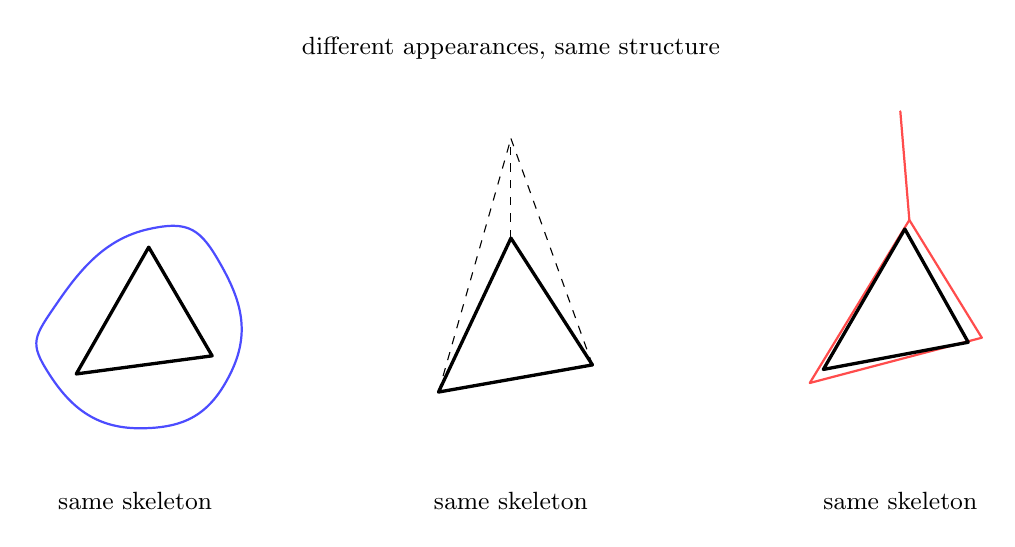
\begin{tikzpicture}[scale=1.15, line join=round]
% left soft form
\draw[thick,blue!70] plot[smooth cycle,tension=0.9] coordinates
  {(-5,0.2) (-4.0,1.0) (-3.2,0.6) (-3.1,-0.6) (-4.1,-1.2) (-5.1,-0.6)};
\draw[very thick] (-4.8,-0.6)--(-4.0,0.8)--(-3.3,-0.4)--cycle;
\node at (-4.15,-2.0) {\small same skeleton};
% center wireframe
\draw[very thick] (-0.8,-0.8)--(0,0.9)--(0.9,-0.5)--cycle;
\draw[dashed] (0,0.9)--(0,2.0);
\draw[dashed] (-0.8,-0.8)--(0,2.0);
\draw[dashed] (0.9,-0.5)--(0,2.0);
\node at (0,-2.0) {\small same skeleton};
% right angular shell
\draw[thick,red!70] (3.3,-0.7)--(4.4,1.1)--(5.2,-0.2)--cycle;
\draw[thick,red!70] (4.4,1.1)--(4.3,2.3)--cycle;
\draw[very thick] (3.45,-0.55)--(4.35,1.0)--(5.05,-0.25)--cycle;
\node at (4.3,-2.0) {\small same skeleton};
% label
\node at (0,3.0) {\small different appearances, same structure};
\end{tikzpicture}
\caption{An idea can look different on the outside while keeping the same inner structure.}
\end{figure}

\section{The Shape That Travels}

A circle\index[words]{circle} is a circle\index[words]{circle} whether it is drawn on paper, traced in sand, or
described in words. The rule ``all points equally far from the center''
works in every case.

When an idea has this kind of stability---when it stays true across many
different materials and situations---that is a sign that you have found
something real.

\begin{quote}\itshape
If you change everything except the rule,
you have not really changed the idea.
\end{quote}

\textbf{Activity:} Pick a simple rule (like ``things fall down''). How many
different places can you find that rule? Does it work in water? In space?
What happens to the rule when the situation changes?

\begin{teachernote}
This chapter develops the idea of invariance\index[keywords]{invariance}. Students are asked to
distinguish between what changes and what stays the same. The triangle\index[words]{triangle}
exercise is not about geometry. It is about identity under transformation.
Students should recognize that size, orientation, and material can change
without changing the underlying rule. Watch for students who focus on
appearance rather than structure. If they say two shapes are different
because they look different, redirect them to the defining rule. The
breaking step (curving a side or adding a fourth side) is important. It
shows that similarity of appearance is not enough; the defining rule must
be preserved. Encourage students to generate their own examples from
music\index[words]{music}, language, or construction. The goal is to generalize invariance\index[keywords]{invariance}
beyond shapes. This chapter prepares students to recognize structure
across domains, which will be essential later.
\end{teachernote}

\section*{Hands-On Demonstration: The Same Shape in Different Forms}

\textbf{What You Need:}
\begin{itemize}
  \item A piece of paper
  \item A pencil
\end{itemize}

\textbf{Step 1: Draw a Simple Shape}

Draw a triangle\index[words]{triangle}. Now write this rule underneath it:

\emph{``A triangle\index[words]{triangle} has three straight sides.''}

\textbf{Step 2: Change the Appearance}

Now draw another triangle, but make it very different. Make it tall and
thin. Make it wide and flat. Turn it upside down. Each one looks different,
but each one still follows the rule.

\textbf{Step 3: Change the Material (In Your Mind)}

Now imagine the same triangle made of wood, drawn in sand, built with
metal beams, or formed by three beams of light. The material changes,
but the rule stays the same.

\textbf{Step 4: Break the Rule}

Now try to draw something that \emph{looks like} a triangle, but does not
follow the rule. Add a fourth side, or curve one of the edges. Now it is
no longer a triangle, even if it looks similar.

\textbf{Step 5: Try With Other Things}

Think about a song played on piano or guitar. A story told out loud or
written down. A building made from wood or steel. What stays the same,
even when everything else changes?

\textbf{Big Lesson:} The skeleton\index[words]{skeleton}\index[keywords]{skeleton (of an idea)} of an idea is what remains when
everything else changes.

% ════════════════════════════════════════════════════════════════════════
\part{How Ideas Become Fast}
% ════════════════════════════════════════════════════════════════════════

\chapter{Why Experts Seem Fast}

\section{Practice Makes Invisible Work}

Have you ever watched an expert\index[words]{expert} do something and thought, ``How does she
do that so fast?'' A chef who chops vegetables without looking. A basketball
player who passes without turning his head. A musician who plays without
reading the notes.

It looks like magic, but it is not. It is practice\index[words]{practice}\index[keywords]{practice}---and practice\index[words]{practice}\index[keywords]{practice} does
something very specific to the brain\index[words]{brain}.

When you practice\index[words]{practice}\index[keywords]{practice} something, your brain\index[words]{brain} learns the rules of that activity
so well that it does not need to think through them anymore. It stores the
whole pattern, already solved, so it can run the solution\index[words]{solution} instantly next
time.

\begin{quote}\itshape
Fast answers are just slow answers that finished early.
\end{quote}

% ── Chapter 5 Figure ─────────────────────────────────────────────────────
\begin{figure}[h!]
\centering
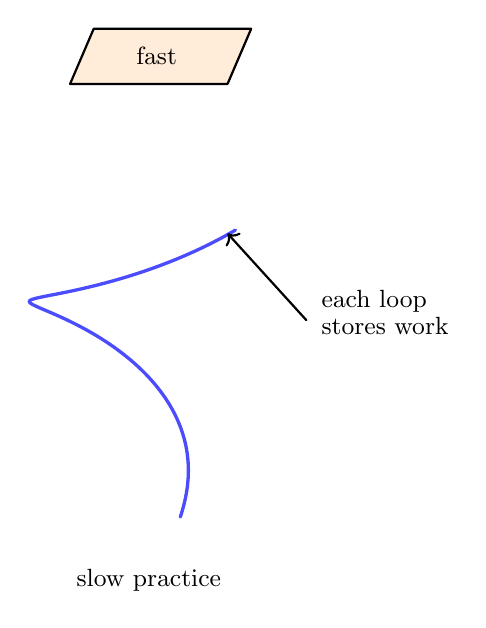
\begin{tikzpicture}[scale=1.0, line cap=round, line join=round]
% spiral
\foreach \t in {0,12,...,300} {
  \pgfmathsetmacro{\r}{0.4 + 0.006*\t}
  \pgfmathsetmacro{\x}{\r*cos(\t)}
  \pgfmathsetmacro{\y}{0.45*\r*sin(\t)}
  \fill[blue!50] (\x,\y + 0.015*\t) circle (0.4pt);
}
\draw[very thick,blue!70,domain=0:300,samples=120,smooth,variable=\t]
  plot ({(0.4 + 0.006*\t)*cos(\t)},
       {0.45*(0.4 + 0.006*\t)*sin(\t) + 0.015*\t});
% top platform
\draw[thick,fill=orange!15] (-1.0,5.5)--(1.0,5.5)--(1.3,6.2)--(-0.7,6.2)--cycle;
\node at (0.1,5.85) {\small fast};
% base label
\node at (0,-0.8) {\small slow practice};
\draw[->,thick] (2.0,2.5) -- (1.0,3.6);
\node[align=left] at (3.0,2.6) {\small each loop \\[-2pt] \small stores work};
\end{tikzpicture}
\caption{Speed grows from many layers of practice stored over time.}
\end{figure}

\section{Work Done Ahead of Time}

Think of it like homework. If you do your homework the night before, you
can answer the question immediately when the teacher asks. If you did not
do your homework, you have to work it out on the spot, which takes much
longer.

What we call ``intuition\index[keywords]{intuition}'' is really homework that you did a long time ago.
Your brain\index[words]{brain} worked out the answer through practice\index[words]{practice} and stored it away. When
the situation appears again, the answer is already there.

\begin{quote}\itshape
Your brain\index[words]{brain} likes to do work ahead of time,
so it can look lazy later.
\end{quote}

\section{What Happens When Things Change}

Here is the tricky part. When you store a solution\index[words]{solution}, you store it for a
particular kind of situation. If the situation changes---if the rules
shift---your stored answer might not work anymore.

Have you ever been very good at one version of a game, and then played a
slightly different version and found yourself making mistakes\index[words]{mistake}? You were
using your old stored answer in a new situation where it did not fit.

That uncomfortable feeling---the moment when your fast thinking is suddenly
wrong---is actually very useful. It tells you that something has changed.
It is the signal to slow down and think carefully again.

\textbf{Big Idea:} Fast thinking is precomputed\index[keywords]{precomputation}. When it stops working, that
is not failure\index[words]{failure}; it is information. Something new has appeared.

\begin{teachernote}
This chapter introduces precomputation. Students often interpret speed as
talent or intuition\index[keywords]{intuition}. The goal is to reframe speed as stored work. Students
should notice the difference between solving a problem and recognizing an
answer. This distinction is central. The video game\index[keywords]{video games} and cooking examples
from the earlier chapter connect naturally here: what felt like ``just
knowing'' was actually accumulated rule storage. Watch for students who
describe fast answers as ``just knowing.'' Ask what changed between the
first and second attempt. Guide them toward the idea that the work was
done earlier. The chapter is successful when students begin to understand
that fluency comes from repeated correct application of rules, not from
guessing.
\end{teachernote}

% ────────────────────────────────────────────────────────────────────────
\chapter{Building Speed Slowly}
% ────────────────────────────────────────────────────────────────────────

\section{The Right Kind of Repetition}

Not all practice builds useful speed. Repeating a mistake\index[words]{mistake} just stores the
mistake\index[words]{mistake} faster. Good practice means working out the correct rule and then
repeating it until it is stored cleanly.

\begin{quote}\itshape
If your answer comes too fast, it might be answering yesterday's question.
\end{quote}

% ── Chapter 6 Figure ─────────────────────────────────────────────────────
\begin{figure}[h!]
\centering
\tdplotsetmaincoords{70}{110}
\begin{tikzpicture}[tdplot_main_coords, scale=1.8, line join=round]
% floor grid
\foreach \x in {0,1,2,3,4,5} {
  \draw[gray!35] (\x,0,0)--(\x,4,0);
}
\foreach \y in {0,1,2,3,4} {
  \draw[gray!35] (0,\y,0)--(5,\y,0);
}
% wall
\fill[red!18] (3,1.4,0)--(3.2,1.4,0)--(3.2,2.8,0)--(3,2.8,0)--cycle;
\fill[red!18] (3,1.4,1.4)--(3.2,1.4,1.4)--(3.2,2.8,1.4)--(3,2.8,1.4)--cycle;
\draw[thick,red!70] (3,1.4,0)--(3.2,1.4,0)--(3.2,2.8,0)--(3,2.8,0)--cycle;
\draw[thick,red!70] (3,1.4,1.4)--(3.2,1.4,1.4)--(3.2,2.8,1.4)--(3,2.8,1.4)--cycle;
\draw[thick,red!70] (3,1.4,0)--(3,1.4,1.4) (3.2,1.4,0)--(3.2,1.4,1.4)
  (3.2,2.8,0)--(3.2,2.8,1.4) (3,2.8,0)--(3,2.8,1.4);
% fast path crash
\draw[ultra thick,blue!70,->] (0.4,2.1,0.05) -- (2.95,2.1,0.05);
\node[blue!70] at (1.4,2.45,0.2) {\small old pattern};
% careful path
\draw[ultra thick,green!50!black,->]
  (0.4,1.2,0.05) .. controls (1.7,1.2,0.05) and (2.2,0.8,0.05) ..
  (3.4,0.8,0.05) .. controls (4.0,0.8,0.05) and (4.2,1.8,0.05) ..
  (4.6,2.2,0.05);
\node[green!50!black] at (4.2,0.4,0.2) {\small slow down and change};
\end{tikzpicture}
\caption{Fast thinking works until the pattern changes; then careful thinking finds a new path.}
\end{figure}

\section{Knowing When to Slow Down}

The most important skill connected to fast thinking is knowing when to stop
using it. Experts\index[words]{expert} are fast---but the best experts\index[words]{expert} also know when a situation
is new enough to need slow, careful thinking.

Slowing down when needed is not a weakness. It is the sign of someone who
understands the limits of their own stored knowledge\index[words]{knowledge}.

\begin{quote}\itshape
The moment you feel sure is sometimes the moment you should check.
\end{quote}

\begin{teachernote}
This chapter introduces the limits of fast thinking. Students learn that
stored patterns are useful only when the situation matches the pattern.
Students should not be discouraged by mistakes. Instead, they should
recognize the mistake as a signal that the pattern has changed. Encourage
students to describe what the mistake felt like. The moment of confusion
is the transition point between fast and slow thinking. The objective is
to build metacognition: students begin to notice when their own thinking
is no longer reliable. This chapter is successful when students learn to
pause and re-evaluate rather than continue applying a failing pattern.
\end{teachernote}

% ════════════════════════════════════════════════════════════════════════
\part{How Ideas Can Fail}
% ════════════════════════════════════════════════════════════════════════

\chapter{When Ideas Break}

\section{Pieces That Do Not Fit}

Sometimes you have a story about how things work, and it mostly makes sense.
But then one day, something does not fit. A prediction turns out to be wrong.
Two parts of what you believed turn out to contradict each other.

This is not a disaster. It is a useful signal. Something in your set of
rules needs to be fixed.

\begin{quote}\itshape
If something cannot exist, that is not a failure.
It is a very clear answer.
\end{quote}

% ── Chapter 7 Figure ─────────────────────────────────────────────────────
\begin{figure}[h!]
\centering
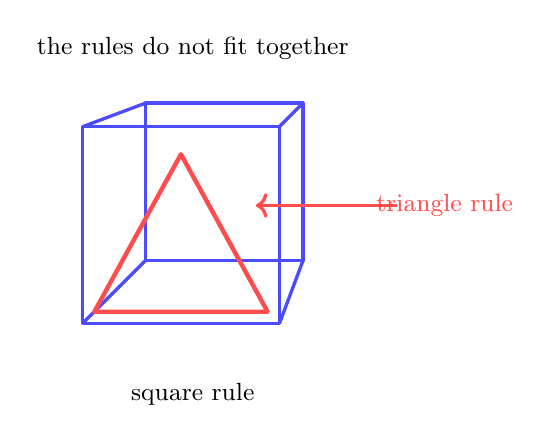
\begin{tikzpicture}[scale=1.0, line join=round]
% impossible frame
\draw[very thick,blue!70] (0,0)--(2.5,0)--(2.5,2.5)--(0,2.5)--cycle;
\draw[very thick,blue!70] (0.8,0.8)--(2.8,0.8)--(2.8,2.8)--(0.8,2.8)--cycle;
\draw[very thick,blue!70] (0,0)--(0.8,0.8) (2.5,0)--(2.8,0.8)
  (2.5,2.5)--(2.8,2.8) (0,2.5)--(0.8,2.8);
% conflicting triangle overlay
\draw[ultra thick,red!70] (0.15,0.15)--(2.35,0.15)--(1.25,2.15)--cycle;
\node[align=center] at (1.4,-0.9) {\small square rule};
\node[align=center,red!70] at (4.6,1.5) {\small triangle rule};
\draw[->,red!70,very thick] (4.0,1.5) -- (2.2,1.5);
\node at (1.4,3.5) {\small the rules do not fit together};
\end{tikzpicture}
\caption{A contradiction happens when two structures demand shapes that cannot both be true at once.}
\end{figure}

\section{The Map That Does Not Match the Territory}

A map is only useful if it matches the real world. When a map is wrong,
you can walk in circles\index[words]{circle} confidently and still get lost.

Ideas are maps. When an idea stops matching reality---when predictions fail,
when pieces disagree---the map needs updating. The real world does not change
to fit your map. The map changes to fit the world.

\section{Fake Answers}

There is another way ideas fail, and it is more subtle. Sometimes we make
an answer \emph{appear} to work by ignoring the parts of reality that
contradict it. We focus only on the cases that fit. We stop testing.

An answer like this feels true but is fragile. It falls apart the moment
someone looks at it from a different angle or applies it to a new situation.
A real answer stays true even when tested hard.

\begin{quote}\itshape
Two ideas that disagree are trying to tell you something.
They are just not being polite about it.
\end{quote}

\textbf{Big Idea:} An idea is strong when it survives being challenged.
An idea is weak when it only seems to work if you never check it carefully.

\begin{teachernote}
This chapter formalizes contradiction\index[words]{contradiction}\index[keywords]{contradiction}. Students encounter situations where
no solution exists under the given rules. The square-with-three-sides task
in the demonstration is intentionally impossible. The goal is for students
to experience impossibility directly rather than being told. Students may
attempt to force a solution. This is useful. It reveals the tendency to
preserve an idea even when it cannot work. Guide students to articulate
why the task cannot be completed. The focus should be on the rules, not
on the drawing. The key shift is recognizing contradiction\index[words]{contradiction}\index[keywords]{contradiction} as information.
It identifies exactly where an idea fails. This chapter prepares students
for repair\index[words]{repair}\index[keywords]{repair (of ideas)} by teaching them how to locate the point of failure.
\end{teachernote}

\section*{Hands-On Demonstration: When Two Things Cannot Both Be True}

\textbf{What You Need:}
\begin{itemize}
  \item A piece of paper
  \item A pencil
\end{itemize}

\textbf{Step 1: Follow the Instructions Carefully}

Draw a shape that follows these two rules: the shape must be a square, and
the shape must have three sides.

\textbf{Step 2: Try to Draw It}

Take a moment and try.

\textbf{Step 3: What Happened?}

You cannot do it. A square has four sides. A three-sided shape is a
triangle. The two rules cannot both be true at the same time.

\textbf{Step 4: Another Example}

Now try to think of a number that is even and odd at the same time. There
is no such number.

\textbf{Step 5: What Do You Do When This Happens?}

When two rules cannot both be true, you must change one of the rules, or
realize one of them is incorrect, or understand that they apply in
different situations.

\textbf{Big Lesson:} When two parts of an idea cannot both be true, you
have found the place where the idea needs to be fixed.

% ────────────────────────────────────────────────────────────────────────
\chapter{How to Fix a Broken Idea}
% ────────────────────────────────────────────────────────────────────────

\section{Finding the Crack}

When something breaks, the most useful thing is to find exactly where the
break is. Not to patch over it with a new guess, but to find the specific
place where the rules stop agreeing.

\begin{quote}\itshape
Fixing one small mistake can save a very big idea.
\end{quote}

% ── Chapter 8 Figure ─────────────────────────────────────────────────────
\begin{figure}[h!]
\centering
\tdplotsetmaincoords{68}{120}
\begin{tikzpicture}[tdplot_main_coords, scale=2.0, line join=round]
% block
\coordinate (A) at (0,0,0);
\coordinate (B) at (2,0,0);
\coordinate (C) at (2,1.4,0);
\coordinate (D) at (0,1.4,0);
\coordinate (E) at (0,0,1.2);
\coordinate (F) at (2,0,1.2);
\coordinate (G) at (2,1.4,1.2);
\coordinate (H) at (0,1.4,1.2);
\draw[thick] (A)--(B)--(C)--(D)--cycle;
\draw[thick] (E)--(F)--(G)--(H)--cycle;
\draw[thick] (A)--(E) (B)--(F) (C)--(G) (D)--(H);
% crack
\draw[ultra thick,red!70,decorate,
  decoration={zigzag,segment length=3pt,amplitude=1pt}]
  (0.9,0,0.6)--(1.0,0.5,0.65)--(0.95,1.0,0.6)--(1.05,1.4,0.65);
% replacement piece
\fill[green!20] (2.6,0.3,0.1)--(3.2,0.3,0.1)--(3.2,1.1,0.1)--(2.6,1.1,0.1)--cycle;
\fill[green!20] (2.6,0.3,0.9)--(3.2,0.3,0.9)--(3.2,1.1,0.9)--(2.6,1.1,0.9)--cycle;
\draw[thick,green!50!black]
  (2.6,0.3,0.1)--(3.2,0.3,0.1)--(3.2,1.1,0.1)--(2.6,1.1,0.1)--cycle;
\draw[thick,green!50!black]
  (2.6,0.3,0.9)--(3.2,0.3,0.9)--(3.2,1.1,0.9)--(2.6,1.1,0.9)--cycle;
\draw[thick,green!50!black]
  (2.6,0.3,0.1)--(2.6,0.3,0.9) (3.2,0.3,0.1)--(3.2,0.3,0.9)
  (3.2,1.1,0.1)--(3.2,1.1,0.9) (2.6,1.1,0.1)--(2.6,1.1,0.9);
\draw[->,very thick] (3.0,1.5,0.6)--(1.3,1.2,0.6);
\node[align=center] at (3.0,-0.25,0.5) {\small replace the bad rule};
\node[align=center] at (1.0,-0.4,0.4) {\small find the crack};
\end{tikzpicture}
\caption{Fixing an idea means finding the weak part and repairing it, not rebuilding everything.}
\end{figure}

\section{Starting from What You Know Is True}

When fixing a broken idea, start from the parts you are most certain of
and rebuild carefully from there. Keep the rules you have tested most.
Let go of the rules you have tested least.

\begin{quote}\itshape
If everything breaks, you probably fixed the wrong part.
\end{quote}

\section{Accepting That Starting Over Is Sometimes Right}

Sometimes the whole structure needs to come down. This is not a failure;
it is actually a very high level of thinking. Only someone who understands
something deeply can tell when the whole structure is wrong, not just a
single detail.

\begin{quote}\itshape
Sometimes an idea grows by unfolding what was already inside it.
\end{quote}

\begin{teachernote}
This chapter introduces repair\index[words]{repair}\index[keywords]{repair (of ideas)}. Students move from identifying failure
to modifying rules so that they become consistent. The bird example is
carefully chosen because it appears correct at first. Students often
accept ``all birds can fly'' without question. The contradiction\index[words]{contradiction} with
penguins creates a need for revision. This should not be resolved
immediately by the teacher. Encourage students to suggest possible fixes.
The correct move is to refine the rule (``most birds can fly'') rather
than discard all related knowledge\index[words]{knowledge}. Watch for overcorrection, where
students discard too much. Guide them to preserve what still works. This
chapter is successful when students begin to see ideas as systems that
can be improved rather than replaced entirely.
\end{teachernote}

% ════════════════════════════════════════════════════════════════════════
\part{How Ideas Show Up in the World}
% ════════════════════════════════════════════════════════════════════════

\chapter{Ideas Everywhere}

\section{The Same Pattern in Different Places}

Here is something remarkable. The same hidden structure shows up in places
that look completely different on the surface.

The way water flows around a rock is related to the way air flows around
an airplane wing. The way a tree grows outward from a center is related to
the way cities grow. The way your heart beats in a rhythm is related to
the way music\index[words]{music} is organized.

None of these things look alike. But they share a structure underneath.
When you have learned to see the structure, you can recognize it anywhere.

\begin{quote}\itshape
If two things look different but behave the same,
you have found something important.
\end{quote}

% ── Chapter 9 Figure ─────────────────────────────────────────────────────
\begin{figure}[h!]
\centering
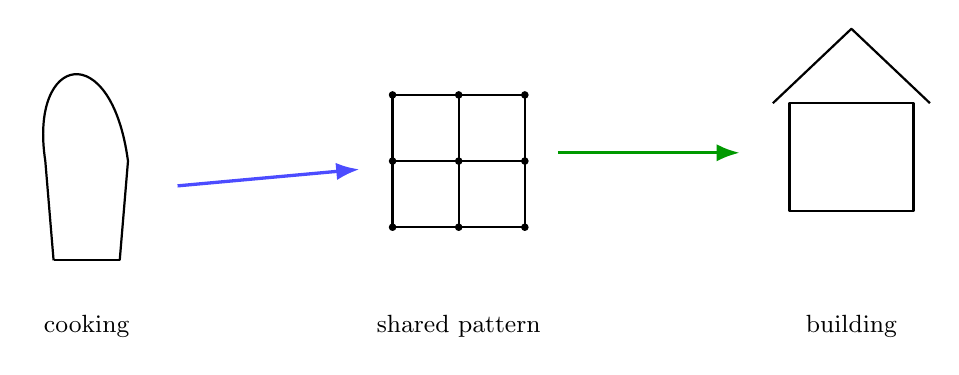
\begin{tikzpicture}[scale=1.05, line join=round, >=Latex]
% left: pot
\draw[thick] (-5,0) .. controls (-5.2,1.3) and (-4.2,1.5) .. (-4.0,0);
\draw[thick] (-4.9,-1.2)--(-4.1,-1.2);
\draw[thick] (-5.0,0)--(-4.9,-1.2) (-4.0,0)--(-4.1,-1.2);
\node at (-4.5,-2.0) {\small cooking};
% center lattice
\foreach \x in {-0.8,0,0.8} {
  \foreach \y in {-0.8,0,0.8} {
    \filldraw[black] (\x,\y) circle (1.1pt);
  }
}
\draw[thick]
  (-0.8,-0.8)--(0,-0.8)--(0.8,-0.8)
  (-0.8,0)--(0,0)--(0.8,0)
  (-0.8,0.8)--(0,0.8)--(0.8,0.8)
  (-0.8,-0.8)--(-0.8,0)--(-0.8,0.8)
  (0,-0.8)--(0,0)--(0,0.8)
  (0.8,-0.8)--(0.8,0)--(0.8,0.8);
\node at (0,-2.0) {\small shared pattern};
% right: house frame
\draw[thick] (4.0,-0.6)--(5.5,-0.6)--(5.5,0.7)--(4.0,0.7)--cycle;
\draw[thick] (3.8,0.7)--(4.75,1.6)--(5.7,0.7);
\node at (4.75,-2.0) {\small building};
% arrows
\draw[->,very thick,blue!70] (-3.4,-0.3)--(-1.2,-0.1);
\draw[->,very thick,green!60!black] (1.2,0.1)--(3.4,0.1);
\end{tikzpicture}
\caption{Different subjects can look different on the surface while sharing the same hidden pattern.}
\end{figure}

\section{Tools That Work in Many Places}

When you learn something truly---not just the surface facts\index[words]{fact} but the deep
rule---you get a tool that works in many situations, not just the one you
learned it in.

Mathematics\index[words]{mathematics} is the most famous example. A rule learned in one place---say,
how to measure the area of a rectangle---turns out to be useful in physics,
in architecture, in music\index[words]{music}, in economics. The rule traveled because it was
a deep rule, not a surface rule.

\section{You Are a Pattern-Finder}

Every time you notice that two different things share a structure, you are
doing the most important work a thinker can do. You are not just learning
facts\index[words]{fact}. You are finding the rules that hold across facts\index[words]{fact}.

That is what science does. That is what art does. That is what any good
thinking does.

\begin{quote}\itshape
Sometimes the same idea is wearing a different job.
\end{quote}

\textbf{Final Big Idea:} Different subjects share hidden structures. When
you find those structures, your knowledge\index[words]{knowledge} in one place becomes useful in
many other places. Ideas are not locked inside one subject. They travel.

\begin{teachernote}
This chapter introduces cross-domain\index[keywords]{cross-domain thinking} structure. Students learn to identify
similar patterns in different contexts. The cooking, building, and game
examples are chosen because they are familiar but appear unrelated. The
objective is for students to recognize a shared structure: gathering
components, combining them, and achieving a goal. Students may initially
focus on surface differences. Redirect attention to the sequence of
actions and their roles. Encourage students to generate their own pairs
of examples. The activity is most effective when the connection is
discovered rather than provided. The key shift is from subject-based
thinking to structure-based thinking. This chapter prepares students to
transfer\index[keywords]{transfer (of knowledge)} knowledge\index[words]{knowledge} across domains, which is essential for independent
problem solving.
\end{teachernote}

\section*{Hands-On Demonstration: The Same Pattern in Different Worlds}

\textbf{What You Need:}
\begin{itemize}
  \item A piece of paper
  \item A pencil
\end{itemize}

\textbf{Step 1: Look at Three Different Activities}

Write down these three things: cooking a meal, building a small structure
like a shelf, and playing a video game\index[keywords]{video games} level. They seem completely different.

\textbf{Step 2: Break Each One Into Steps}

For cooking: gather ingredients, combine them, apply heat.
For building: gather materials, assemble parts, secure them.
For the game: collect resources, use tools, complete the objective.

\textbf{Step 3: Compare the Structure}

Now look closely. Each one follows a similar pattern: start with pieces,
combine them in the right way, reach a goal. The details are different,
but the structure is the same.

\textbf{Step 4: Find Your Own Example}

Think of two things that seem unrelated, like drawing a picture and solving
a math problem. Try to find the shared pattern underneath.

\textbf{Big Lesson:} When you learn a deep pattern, you are not just
learning one thing---you are learning something that applies everywhere.

% ────────────────────────────────────────────────────────────────────────
\chapter{What This Means for You}
% ────────────────────────────────────────────────────────────────────────

\section{Learning Is Rule Collection}

Every time you learn something new, you are adding a rule to your collection.
The more rules you collect from more different places, the richer your
collection becomes---and the more likely it is that someday, your rules will
all point to the same answer at the same time.

\begin{quote}\itshape
You already know more rules than you think.
They are just waiting to meet each other.
\end{quote}

% ── Chapter 10 Figure ─────────────────────────────────────────────────────
\begin{figure}[h!]
\centering
\tdplotsetmaincoords{70}{115}
\begin{tikzpicture}[tdplot_main_coords, scale=1.9, line join=round]
% target structure center
\coordinate (A) at (0,0,0);
\coordinate (B) at (1.3,0,0);
\coordinate (C) at (1.3,1.2,0);
\coordinate (D) at (0,1.2,0);
\coordinate (E) at (0.4,0.3,1.1);
\coordinate (F) at (1.7,0.3,1.1);
\coordinate (G) at (1.7,1.5,1.1);
\coordinate (H) at (0.4,1.5,1.1);
\draw[ultra thick] (A)--(B)--(C)--(D)--cycle;
\draw[ultra thick] (E)--(F)--(G)--(H)--cycle;
\draw[ultra thick] (A)--(E) (B)--(F) (C)--(G) (D)--(H);
\node at (0.9,-0.45,0) {\small your idea};
% incoming pieces
\draw[thick,blue!70]
  (-2.6,0.2,0.2)--(-1.8,0.2,0.2)--(-1.8,1.0,0.2)--(-2.6,1.0,0.2)--cycle;
\node[blue!70] at (-2.2,-0.3,0.2) {\small game rule};
\draw[thick,red!70]
  (0.2,-2.0,0.2)--(1.0,-2.0,0.2)--(0.6,-1.2,0.2)--cycle;
\node[red!70] at (0.6,-2.45,0.2) {\small cooking rule};
\draw[thick,green!50!black]
  (3.0,0.2,0.2)--(3.8,0.2,0.2)--(3.8,1.0,0.2)--(3.0,1.0,0.2)--cycle;
\node[green!50!black] at (3.4,-0.3,0.2) {\small building rule};
% arrows
\draw[->,very thick,blue!70] (-1.7,0.6,0.2)--(-0.1,0.6,0.2);
\draw[->,very thick,red!70] (0.6,-1.1,0.2)--(0.8,-0.05,0.2);
\draw[->,very thick,green!50!black] (2.95,0.6,0.2)--(1.9,0.6,0.2);
\node at (0.9,2.0,0.7) {\small combine rules from many places};
\end{tikzpicture}
\caption{Strong ideas are built by combining rules from different places into one working structure.}
\end{figure}

\section{Discovery Feels Like Recognition}

When that happens---when your rules all line up and the answer arrives---
it will not feel like you invented something. It will feel like you finally
saw something that was there all along.

That is what discovery\index[keywords]{discovery} is. Not invention, but recognition\index[words]{recognition}\index[keywords]{recognition}. Not making
something new from nothing, but finding the shape that was always there,
waiting for you to accumulate enough rules to see it.

\section{How to Prepare}

Learn rules from many different places, not just one subject. Look for
patterns that show up more than once, in more than one place. When an idea
breaks, find the crack---do not cover it over. Practice until good rules
become fast, then stay ready to slow down when something new appears.
Remember: the click of recognition\index[words]{recognition}\index[keywords]{recognition} is not luck. It is what happens after
a lot of careful rule collection.

\begin{quote}\itshape
Good ideas are not built from nothing.
They are built from things that were already almost connected.
\end{quote}

\begin{quote}\itshape
It might have been a small idea.
Or it might have been a folded one.
\end{quote}

\begin{teachernote}
This final chapter integrates all previous concepts into a generative
process. Students are no longer identifying patterns; they are constructing
ideas by combining rules from different domains. The design task is
intentionally open-ended. Students should experience both the freedom and
the constraint\index[keywords]{constraint} of working within multiple rules. Encourage iteration. The
first design will often contain conflicts or unnecessary complexity. This
is expected. Guide students through testing, simplifying, and refining
their ideas. Each step corresponds to earlier chapters: compatibility,
abstraction, and repair\index[words]{repair}\index[keywords]{repair (of ideas)}. The objective is for students to recognize that
idea creation is a structured process, not a spontaneous event. This
chapter is successful when students can describe how their idea changed
as they tested and improved it.
\end{teachernote}

\section*{Hands-On Demonstration: Building an Idea from Many Places}

\textbf{What You Need:}
\begin{itemize}
  \item A piece of paper
  \item A pencil
\end{itemize}

\textbf{Step 1: Pick a Simple Goal}

Choose something to design: a simple game, a small structure like a fort
or a shelf, or a recipe.

\textbf{Step 2: Gather Rules from Different Places}

Write down rules from at least three different areas. From games: players
take turns, there are goals. From building: it must be stable, it needs
support. From cooking: steps must happen in order, ingredients combine.

\textbf{Step 3: Combine the Rules}

Try to design your idea using all of these rules at once. For example:
a game where players build something step by step, and each move must
keep the structure stable.

\textbf{Step 4: Check for Problems}

Ask yourself: do any of the rules conflict? Does anything not work when
you try to follow all the rules? If something breaks, go back and fix
the rule.

\textbf{Step 5: Simplify}

Now remove anything that is not necessary. Keep only the parts that make
the idea work.

\textbf{Step 6: Test Your Idea}

Explain your idea to someone else, or imagine someone using it. Does it
still work? Does it make sense? If not, find the weak part and fix it.

\textbf{What Happened?} You did not guess an idea. You built it by combining
rules, checking them, and refining them.

\textbf{Final Big Lesson:} Ideas are not magic. They are built from rules.
The more carefully you collect, test, and combine those rules, the more
powerful your ideas become.


% ════════════════════════════════════════════════════════════════════════
\backmatter
% ════════════════════════════════════════════════════════════════════════

\printindex[keywords]

\printindex[words]

\end{document}
